\section{Hyperbolic function definitions}
\subsection{$\sinh x$}
\begin{description}
    \item[Definition] $\sinh x = \dfrac{e^x-e^{-x}}{2}$
    \item[Domain] $x \in \Rset$
    \item[Range] $\sinh x \in \Rset$
    \item[Asymptotes] $x\rightarrow +\infty$, $y\rightarrow\dfrac{e^x}{2}$; $x\rightarrow -\infty$, $y\rightarrow -\dfrac{e^{-x}}{2}$
    \item[x-intercept] $(0,0)$
    \item[y-intercept] $(0,0)$
\end{description}

\subsection{$\cosh x$}
\begin{description}
    \item[Definition] $\cosh x = \dfrac{e^x+e^{-x}}{2}$
    \item[Domain] $x \in \Rset$
    \item[Range] $\cosh x \geq 1$
    \item[Asymptotes] $x\rightarrow +\infty$, $y\rightarrow\dfrac{e^x}{2}$; $x\rightarrow -\infty$, $y\rightarrow\dfrac{e^{-x}}{2}$
    \item[x-intercept] No
    \item[y-intercept] $(0,1)$
\end{description}

\subsection{$\tanh x$}
\begin{description}
    \item[Definition] $\tanh x = \dfrac{\sinh x}{\cosh x}=\dfrac{e^x-e^{-x}}{e^x+e^{-x}}$
    \item[Domain] $x \in \textbf{R}$
    \item[Range] $-1 < \tanh x < 1$
    \item[Asymptotes] $x\rightarrow +\infty$, $y\rightarrow 1$; $x\rightarrow -\infty$, $y\rightarrow -1$
    \item[x-intercept] $(0,0)$
    \item[y-intercept] $(0,0)$
\end{description}

\subsection{Function graphs}
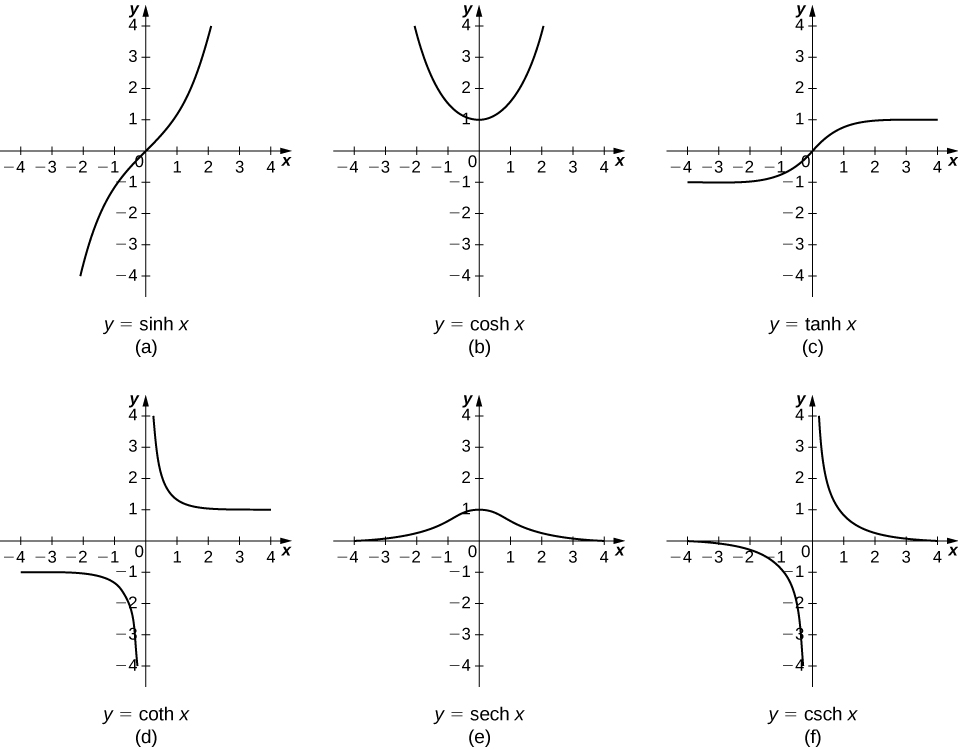
\includegraphics[width=\linewidth]{images/hyperbolic_graphs}

\section{Inverse hyperbolic functions}
\begin{itemize}
    \item $\arsinh x = \ln \left[x+\sqrt{x^2+1}\right]$
    \item $\arcosh x = \ln \left[x+\sqrt{x^2-1}\right] \:\: (x \geq 1)$
    \item $\artanh x = \ln \left[\dfrac{1+x}{1-x}\right] \:\: (-1 < x < 1)$
\end{itemize}

\subsection{Proof}
\begin{example}
    Show that $\arsinh x = \ln \left[x+\sqrt{x^2+1}\right]$
\end{example}

\begin{solution}
    Let $y=\arsinh x$
    \begin{align*}
        \sinh y               & = x                    \\
        \dfrac{e^y-e^{-y}}{2} & = x                    \\
        e^y-e{-y}             & = 2x                   \\
        e^{2y} - 1            & = 2x e^y               \\
        (e^y-x)^2             & = x^2 + 1              \\
        e^y                   & = x \pm \sqrt{x^2 + 1}
    \end{align*}
    $e^y = x + \sqrt{x^2 + 1}$ \text{since $\sqrt{x^2 + 1} > 0$ so it makes $e^y$ negative which is impossible}\\
    Hence $y = \ln \left[x+\sqrt{x^2+1}\right]$ so $\arsinh x = \ln \left[x+\sqrt{x^2+1}\right]$
\end{solution}

\begin{remark}
    Prove these identities by finding value of $e^y$ in quadratic equations, think about domain when deciding the sign before the square root
\end{remark}

\subsection{Graphs}
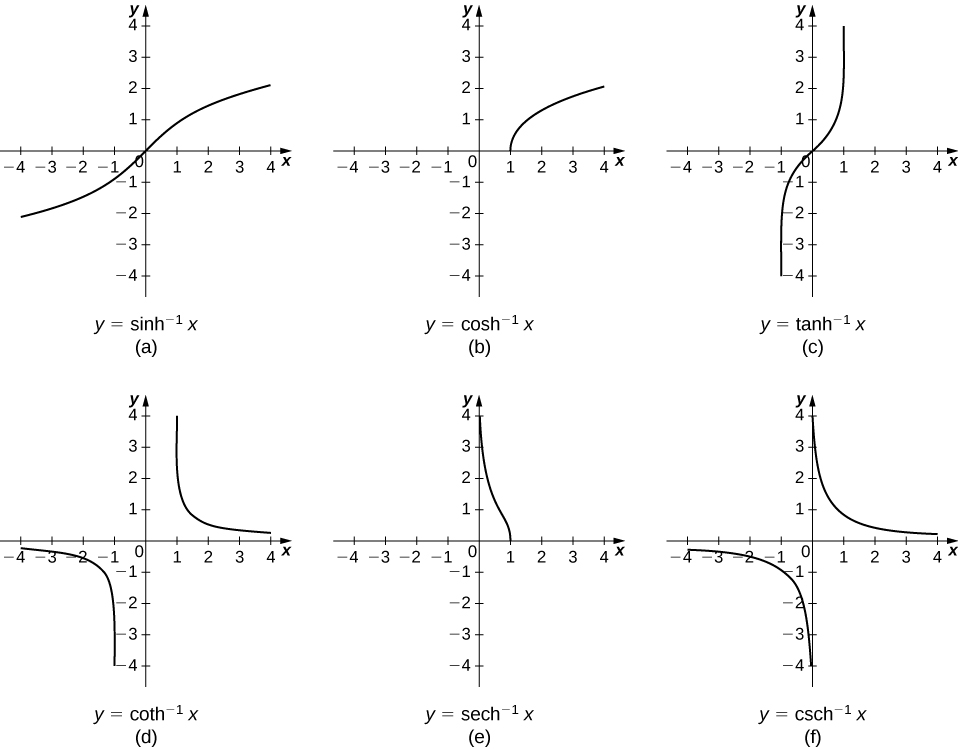
\includegraphics[width=\linewidth]{images/hyperbolic_inverse_graphs}



\section{Identities of hyperbolic functions}
Similar to trigonometric identities:
\begin{itemize}
    \item $\tanh x = \dfrac{\sinh x}{\cosh x}$
    \item $\cosh^2 x - \sinh^2 x = 1$
    \item $\tanh^2 x + \sech^2 x= 1$
    \item $\coth^2 x - \csch^2 x = 1$
\end{itemize}

\subsection{Addition}
\begin{itemize}
    \item $\sinh(x+y)=\sinh x \cosh y + \sinh y \cosh x$
    \item $\cosh(x+y)=\cosh x \cosh y + \sinh x \sinh y$
    \item $\tanh(x+y) = \dfrac{\sinh(x+y)}{\cosh(x+y)} = \dfrac{\sinh x \cosh y + \sinh y \cosh x}{\cosh x \cosh y + \sinh x \sinh y} = \dfrac{\frac{\sinh x}{\cosh x}+\frac{\sinh y}{\cosh y}}{1 + \frac{\sinh x \sinh y}{\cosh x \cosh y}}=\dfrac{\tanh x + \tanh y}{1 + \tanh x \tanh y}$
\end{itemize}

\subsection{Double angle}
\begin{itemize}
    \item $\sinh 2x = 2\sinh x \cosh x$
    \item $\cosh 2x = \cosh^2 x + \sinh^2 x = 2\cosh^2 x - 1 = 2\sinh^2 + 1$
    \item $\tanh 2x = \dfrac{2\tanh x}{1 + \tanh^2 x}$
\end{itemize}

\subsection{Power descending}
\begin{itemize}
    \item $\sinh^2 x = \dfrac{\cosh 2x - 1}{2}$
    \item $\cosh^2 x = \dfrac{\cosh 2x + 1}{2}$
\end{itemize}


\section{Calculus with hyperbolic functions}
\subsection{Differentiation}
\[(\sinh x)'=\cosh x\]
\[(\cosh x)'=\sinh x\]
\[(\tanh x)'=1-\tanh^2 x = \sech^2 x\]
\[(\csch x)'=-\coth x \csch x\]
\[(\sech x)'=-\sech x \tanh x\]
\[(\coth x)'=-\csch^2 x\]
\[(\arsinh x)' = \dfrac{1}{\sqrt{1+x^2}}\]
\[(\arcosh x)' = \dfrac{1}{\sqrt{x^2-1}}\]
\[(\artanh x)' = \dfrac{1}{1-x^2}\]


\subsection{Integration}
\[\int\sinh x \dx = \cosh x + c\]
\[\int\cosh x \dx = \sinh x + c\]
\[\int \tanh x \dx = \ln |\cosh x| + c\]
\[\int \coth x \dx = \ln |\sinh x| + c\]
\[\int \sech x \dx = \ln |-\sech x + \tanh x| + c = \ln \left|\tan\left(\frac{1}{2}x+\frac{1}{4}\pi \right)\right| + c\]
\[\int \csch x \dx = -\ln|\csch x + \coth x| + c\]
\[\int \sinh^2 x \dx = \int \frac{\cosh 2x - 1}{2} \dx = \frac{\sinh 2x - 2x}{4} + c\]
\[\int \cosh^2 x \dx = \int \frac{\cosh 2x + 1}{2} \dx = \frac{\sinh 2x + 2x}{4} + c\]
\[\int \tanh^2 x \dx = \int 1-\sech^2 x \dx = x - \tanh x + c\]
\[\int \coth^2 x \dx = \int 1+\csch^2 x \dx = x - \coth x + c\]
\[\int \sinh x \cosh x \dx = \int \frac{\sinh 2x}{2} \dx = \dfrac{\cosh 2x}{4} + c\]
\[\int \tanh x \sech x \dx = -\sech x + c\]
\[\int \coth x \csch x \dx = -\csch x + c\]
\[\int \frac{1}{\sqrt{x^2-a^2}} \dx= \arcosh \left(\frac{x}{a}\right) + c = \ln \left(x + \sqrt{x^2-a^2}\right) + c \:\:  (x>a)\]
\[\int \frac{1}{\sqrt{a^2+x^2}} \dx= \arsinh \left(\frac{x}{a}\right) + c = \ln \left(x + \sqrt{x^2+a^2}\right) + c \]
\[\int \frac{1}{a^2-x^2} \dx=\frac{1}{a}\artanh \left(\frac{x}{a}\right) + c = \frac{1}{2a}\ln \left|\frac{a+x}{a-x}\right| + c\]
